%\chapter{How to Use Sombrero}
\section{User Mode}
\subsection{What is User Mode?}

  If you are logged in as a simple user, you are considered to be in user mode. In user mode you are not able configure the status of devices and the user  profile properties of others. The status of devices can be changed through clicking. An explanation of every widget will follow later on. The profile properties can be set using the edit user form.

  Sombrero was built to make controlling your house very easy, but to use it properly you first have to understand the concept behind it. A house consists of floors. Floors consist of rooms and in rooms there are devices. You can structure your devices your way, each device is represented by a widget contained in a room. This structuring can only be done in admin mode. To access your devices you can use the tree view sidebar positioned on the left side.

  When you are logged in as a user the layout of the sombrero web page is split into 3 parts. On the left you see the tree view sidebar. The favorites bar is positioned on the top of the page. You can use it to quickly access widgets you use often. On the right side of the page there is some space left. This space is reserved for the widgets in their respective rooms.

  \begin{figure}[h]
  \centering
  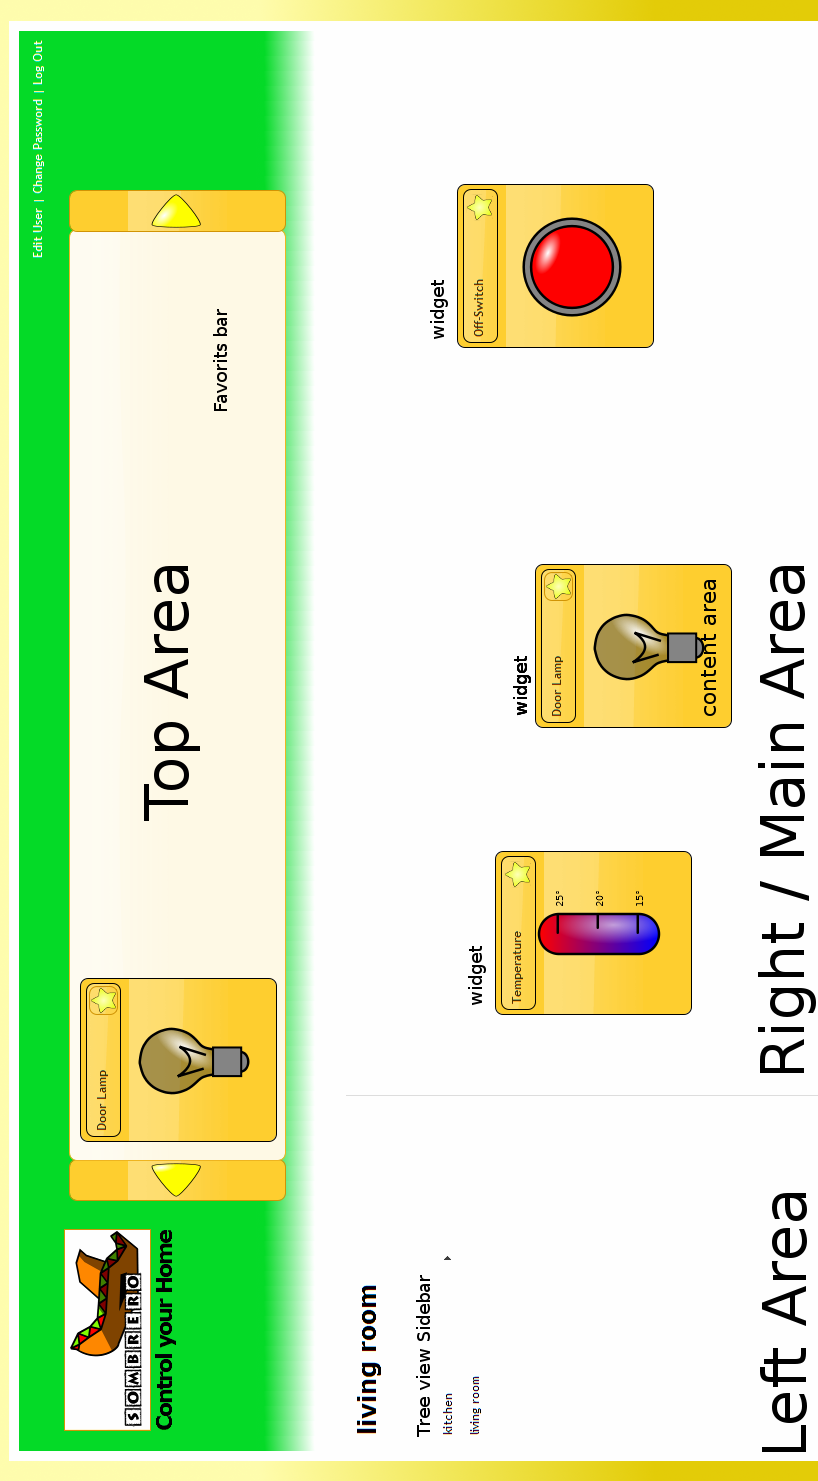
\includegraphics[width=0.80\linewidth]{room3.png}
  %\input{room3}
  \caption{room view structure}
  \label{fig:roomview}
  \end{figure}

  \clearpage
\subsection{Favorites Bar}
  This widget allows you to collect your favorite widgets and quickly access them in every room. The Favorites Bar is also called widget container, because you can add sombrero widgets of almost any kind to it. The content of the Bar stays in the same in every room, so with this widget you can access widgets from another room without being in that room. To add a widget to the Favorites Bar you have to click on the star at the top of the widget. By clicking it again the widget will vanish from the Bar.

\subsection{Tree view Sidebar}
  The tree view sidebar was designed to make navigation between rooms seamless and easy. Just by clicking on the room's name you switch to this room and the tree view sidebar gets updated and displays the rooms in the chosen room. If it has no rooms in it the neighbors are shown. By clicking on the arrow right of the the room name you can switch to the respective room view without loading its content.

  When you navigate into a room which contains rooms, you can go back to the view of the neighbor rooms by clicking the back button on the bottom of the tree view sidebar. Every room has its own URL, so it's possible to bookmark your favorite rooms.

\subsection{Sombrero widgets}
    All widgets that are positioned in the right area of the layout are capable of the following features:
    \begin{itemize}
        \item \textbf{dragging}
            Every Sombrero widget can be dragged in the bounds of the right area of the layout. The position is saved automatically after you drag a widget to a new position.
        \item \textbf{clicking}
            Sombrero widgets are split into two parts. On the top there is the title bar with the name of the widget. Under the title bar there is the content area, containing a selfmade picture of the device the widget represents. By clicking this picture you can change the status or send a command.
        \item \textbf{adding as a favorite}
            The title bar also contains a Star button. By clicking it you add the respective widget to the Favorites Bar and by clicking it again it gets removed. When a widget is up in the Favorites Bar it can also be removed by clicking the Star button of the widget in the Bar. Widgets in the Bar can be used in the same way as if they were down in the right area of the layout.
    \end{itemize}
\subsection{Room Link}
  \begin{figure}[h]
  \centering
  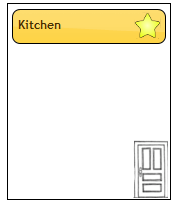
\includegraphics{roomlink.png}
  %\input{roomlink}
  \caption{Room Link}
  \label{fig:roomlink}
  \end{figure}

    This widget is the only one without KNX/EIB functionality. By clicking the picture in the content area of the widget the site will reload and you will find yourself in another room. The Super User has the ability to set a picture for this widget, for example the room the widget links to.
    \clearpage
\subsection{Roller Blind}
  \begin{figure}[h]
  \centering
  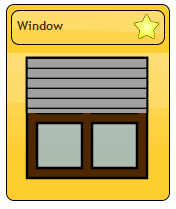
\includegraphics{rollo.png}
  %\input{rollo}
  \caption{Roller Blind}
  \label{fig:rollo}
  \end{figure}

    The Roller Blind is a KNX/EIB device widget. It allows you to control Roller Blinds just by clicking on the Roller Blind. To change state more intuitive, you can move your mouse up and down while it's pressed and the state in which it is in after you released the mouse will be saved.
    \clearpage
\subsection{Temperature actuator}
  \begin{figure}[h]
  \centering
  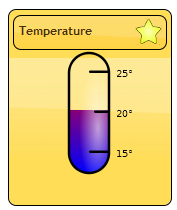
\includegraphics{temperature.png}
  %\input{temperature}
  \caption{Temperature actuator}
  \label{fig:temperature}
  \end{figure}

    This widget is a KNX/EIB device widget and can be used to change temperature of a temperature actuator by clicking the picture in the content area of the widget. To change state more intuitive, you can move your mouse up and down while it's pressed and the state in which it is in after you released the mouse will be saved.
    \clearpage
\subsection{Dimmer}
  \begin{figure}[h]
  \centering
  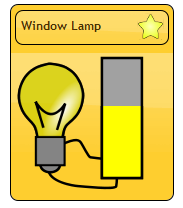
\includegraphics{dimmer.png}
  %\input{dimmer}
  \caption{Dimmer}
  \label{fig:dimmer}
  \end{figure}

    This widget is a KNX/EIB device widget and it is able to change the amount of light emitted from a dimmer by clicking on to the picture in the content area of the widget. To change state more intuitive, you can move your mouse up and down while it's pressed and the state in which it is in after you released the mouse will be saved.
    \clearpage
\subsection{Lamp}
  \begin{figure}[h]
  \centering
  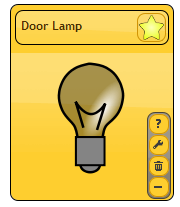
\includegraphics{lamp.png}
  %\input{lamp}
  \caption{Lamp}
  \label{fig:lamp}
  \end{figure}

    The Lamp is a KNX/EIB device widget. It allows you to turn lamps on and off by clicking on to the picture in the content area.
    \clearpage
\subsection{Switch}
  \begin{figure}[h]
  \centering
  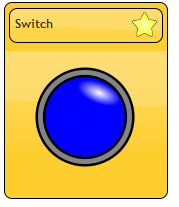
\includegraphics{switch.png}
  %\input{switch}
  \caption{Switch}
  \label{fig:switch}
  \end{figure}

    This widget exists in 3 forms:
    \begin{itemize}
        \item \textbf{Switch}
            With the Switch you can change the state of the device connected to it by clicking on the picture in the content area.
        \item \textbf{Switch Off}
            The Switch Off widget is able to turn the device connected to it off by clicking on the picture in the content area.
        \item \textbf{Switch On}
            The Switch On widget is able to turn the device connected to it on by clicking on the picture in the content area.
    \end{itemize}